%&tex
\chapter{Introduction}

	Computer vision is the scientific endeavour to algorithmically understand patterns in images. Structures and processes in the physical world interact in complex ways to generate an image, the image acts as a mirror, in which these elements of the world are reflected and leave patterns.
	To recognize these patterns in an image, means to use this mirror as a window to observe the reality lurking behind it, \ie to measure the causal elements that contributed to the image generation.
	Formally this can be posed as an inference problem: a number of latent variables $\mathbf{z_1}\ldots\mathbf{z_N}$ interacted in certain ways to cause the image $\mathbf{x}$. An inference algorithm aims at recovering these variables from the observation, \ie the image. This recoveries can be seen as an estimate for or a representation of the true latent variables $\mathbf{z_i}$. A graphical depiction is shown in figure \ref{fig:causal}.
	\begin{figure}[ht]
		\centering
		% 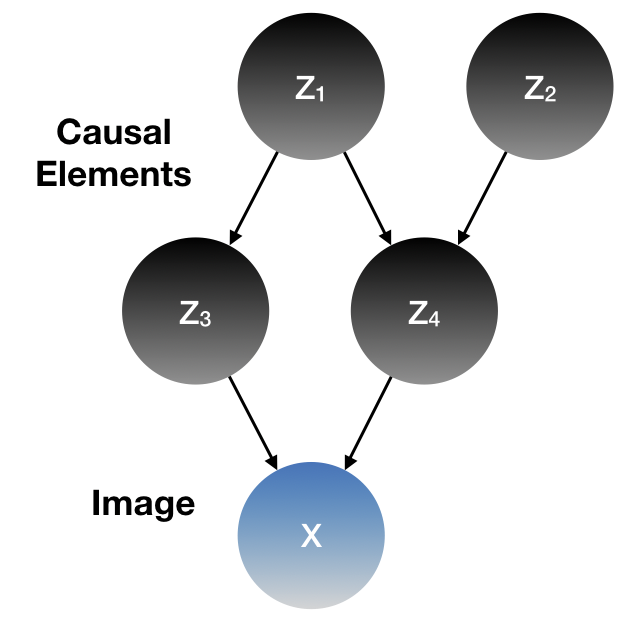
\includegraphics[trim={0cm 0cm 0cm 0cm},clip, width=.3\linewidth]{fig/causal}
		\begin{tikzpicture}
			% Define nodes
			\node[obs]                               (x) {$\mathbf{x}$};
			\node[latent, above=of x, xshift=-1.2cm] (z1) {$\mathbf{z_3}$};
			\node[latent, above=of x, xshift=1.2cm]   (z2) {$\mathbf{z_4}$};
			\node[latent, above=of z1, xshift=-1.2cm] (z3) {$\mathbf{z_1}$};
			\node[latent, above=of z1, xshift=1.2cm]  (z4) {$\mathbf{z_2}$};

			% Connect the nodes
			\edge {z1,z2} {x} ; %
			\edge {z3,z4} {z1} ; %

			% Plates
			% \plate {yx} {(x)(y)} {$N$} ;
			% \plate {} {(w)(y)(yx.north west)(yx.south west)} {$M$} ;
		\end{tikzpicture}
		\caption{Causal elements $\mathbf{z_i}$ contributing to generation of image $\mathbf{x}$}
		\label{fig:causal}
	\end{figure}
	Typically, objects appear in an intricated interaction of many factors of variation.
	For example, given the object class of people, variation can be in visual appearance such as the persons clothing or skin color or variation in geometric shape determined by a persons pose or body physique.
	%
	In order to gain a conceptual understanding of the world, disentangling the underlying factors of variation is a crucial step, as has been argued in numerous works,~\cite{Desjardins2012dr, Bengio2013rep, Chen2016infogan, Higgins2016betavae, Eastwood2018dr}.
	%
	For articulated object classes the most prominent factors are geometric shape and visual appearance.
	Disentangling these factors is a difficult problem due to the intricated interplay of shape and appearance under articulation.
	The complexity enters, as a variation in shape is a change of the images domain rather than a change of its values~\cite{Shu:2018ua}.
	Consider a person raising his arm: the color and texture of his pullover sleeve intrinsically does not change, but appears at a different location in the image. An efficient model for shape should cover all possible states of the object and preserve the local linkage to its intrinsic appearance.

	Finding an abstract image representation, can be framed as a problem of understanding, such that an image representation contains the states of the factors that led to the image including objects and the physical states of objects.
	A factorized representation should then represent each causal element and its state individually, in a disentangled manner: A change in the real causal element should correspond to an equivalent change in the abstract representational factor, while leaving the other factors, that represent other causes, unchanged.
	% Capturing the causal elements that generate an image is a long-standing goal of computer vision and is driving the search for image representations which disentangle these causal factors from each other.
	On the one hand there are pragmatic reasons to aim at extracting disentangled factors from images: to successfully transfer a representation between different tasks, typically only a few factors are relevant \cite{Bengio:2013bu}.
	Efficient transfer and multi-task learning should account for this.
	On the other hand, learning to capture external mechanisms in appropriate internal representations, can be seen as a goal in its own.
	It enables machines to reason about the world \cite{Pearl:2018im}.
	In addition, once disentangled, a factor can be manipulated individually to make a targeted change.
	Thought experiments like \textit{"imagine, how ridiculous you would look, if you wore that hot pants"} are managable tasks for human imagination, but are out of the league for currently used generative image models \cite{Goodfellow:2014td, Kingma:2013tz}, that typically rely on uninterpretable vector spaces with entangled dimensions.
	In the sense of generative modelling, disentangling factors could as well lead the way from a science of images to a science of imagination \cite{Mahadevan:2018tz}.

	% \note{Data-driven algorithms for pattern recognition good recently}
	% \note{how much and how to incorporate prior knowledge}
	% \note{is this necessary, theoretical arguments against}
	% \begin{itemize}
		% \item Computer vision: automatically discern patterns, that reflect structures in physical world
		% \item Why disentangle: detect causal factors to image
		% \item Pragmatic reason: efficient transfer learning, multi-task learning
		% \item Philosophical reason: build machines that understand mechanisms, reason about world \cite{Pearl:2018im}
		% \item Targeted changes $\rightarrow$ thought experiments; not possible for e.g. GAN, VAE\ \textit{"imagine, ..."}\ science of images $\Rightarrow$ science of imagination \cite{Mahadevan:2018tz}.
	% \end{itemize}

	% How Disentangle?
	But how to learn a disentangled representation from scratch, \ie from pure data?
	As we will find out, disentangling causal factors from raw image data, without any side information is impossible theoretically and can only work based on statistical assumptions.
	Lets consider an example to illustrate this point:
	Statistical residues -> will depends on statistical nature of data (e.g. Gaussian with two dimensions P(s, a)
	current machine learning: association, probability distribution modeling.
	% from pure image data without any further assumptions the information about the world will not be learned, because the information does not exist in the data.


	How do humans disentangle?
	1. association: "conditioning"
	2. Apart from pure association -> access to video information
	e.g. video information: how do objects behave across time?

	3. Learning by interacting: knowing change by changing.
	second rung on causal ladder (Pearl): intervention. (, acting) What happens if I do?
	P(s, do(a))
	Others: counterfactual (imagining), association.
	In humans e.g. egomotion cues: how does image on retina change if I move.


	How disentangle?
	change factor -> image change equivariantly, leave others invariant
	-> equivariance, invariance

	change can be mimicked artificially
Intelligent pattern recognition algorithms, fuelled by sensory data as learning material alone, may ultimately drive the way to a full-blown artificial intelligence, reasoning about the world on its own. - That is the reasoning behind data-driven and assumptionless machine learning approaches that have conquered several research communities.
	A theoretical objection to driving-only-with-data comes from the causal literature: For an understanding of the world, an algorithm needs to model causal processes, that cause an image to be generated.

\section{Contributions I}
	\textbf{Hypothesis}: learning shape requires abstracting away appearance -> hence disentangling
	\textbf{Hypothesis \emph{ii)}}: learning disentanglement from pure data is fundamentally constrained. need to take causal literature into account -> disentangling causal factors will need assumptions on causal model and/or interventional/interactional data (instead of raw data).
	% need to interact with the world, need to change, need to model physical reality -> image transformations, analyis-by-synthesis
	\begin{itemize}
		\item validate and evaluate method developed by Lorenz \etal\ 2018 for disentangling
		\item overview over state-of-the-art disentangling, analysis of future directions
		\item explain method in context to these
		\item evaluate unsupervised shape learning:
			\begin{itemize}
				\item human faces, bodies (CelebA, Human3.6M)
				\item animal faces, bodies (cats, dogs, birds)
				\item composite objects (dancing pair)
			\end{itemize}
		\item make own video dataset
			\begin{itemize}
				\item for disentangling human pose and appearance (heidelbergpose)
				\item for articulated animal video (dogs)
				\item for composite object (pair dancing salsa)
			\end{itemize}
		\item ablation study (reconstruction, equivariance loss, transformations)
		\item qualitative comparison to non-disentangling composite shape learning (Zhang)
		may be a petty detail or a simple hack/trick (reconstruction on other image) but makes all the difference in terms of causal information
		\item evaluating disentanglement
			\begin{itemize}
				\item reID
				\item pose estimation
			\end{itemize}
	\end{itemize}
	result: soa in shape learning, (first) unsupervised disentangling of articulated shape and appearance

